\newpage
\mysection{Trees}

A graph is an ordered pair \textbf{\emph{G = (V, E)}} comprising a set \textbf{\emph{V}} of vertices, (aka: nodes or points) together with a set \textbf{\emph{E}} of edges, (aka: arcs or lines).\\

A tree is an \gls{undgraph} in which any two vertices are connected by exactly one path. In other words, any \gls{acyclic} connected graph is a tree.\\

Below is a directory tree. This is a tree that represents a portion of a file system on pretty much any operating system. It's a generic representation of a folder hierarchy, displaying subfolders, and files in folders. Notice that there is no restriction on the number of children. Nodes have from 1-4 children, and could have many more depending on how many items a folder were to contain. All trees represent relationships between items, this tree happens to represent folders and files. In academia we tend to lean toward very defined tree's (Binary Search Tree, \gls{btree}\supcite{Btree}, \gls{rtree}\supcite{Rtree}, \gls{marytree}\supcite{marytree}, \gls{trietree}\supcite{Trie}, and many more.) but these tree are nothing without the algorithms that define their properties and behaviors. This section is just to label components of generic trees. We will get into specifically defined trees later. 

\mysubsection{Tree Vocab}

\begin{center}
	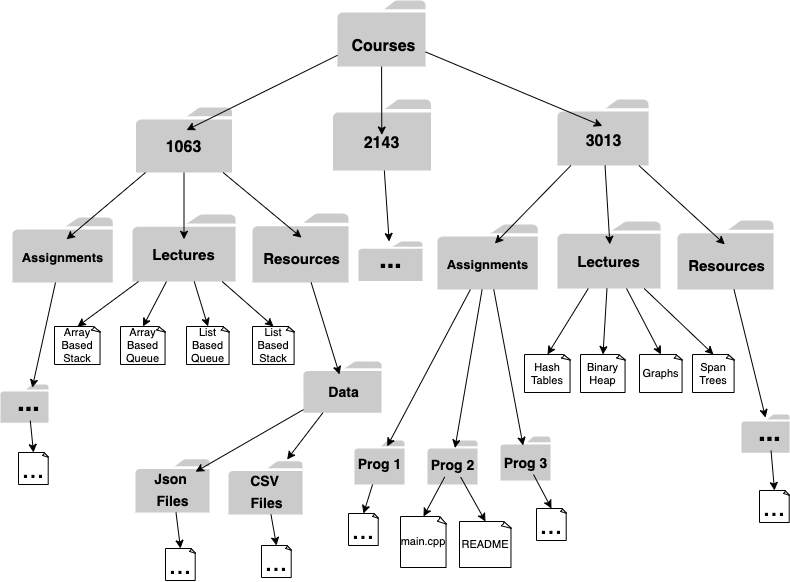
\includegraphics[scale=.45]{images/directory_structure_tree.png}
\end{center}

\begin{center}
	\begin{tabular}{p{0.1\textwidth} p{0.85\textwidth} }
		
		\textbf{Node}      &   
		A node is a fundamental part of a tree. It should contain information. Occasionally 
		all or part of the nodes data is called a  ``key.''  The key is a unique value we 
		use to perform comparisons when finding the proper location to place the node in the 
		tree. The node is not limited to storing only a key, in fact in the real world, it will
		store much more information in addition to the "key". Pretty much only in the classroom and
		books do we find trees that store  only "keys" (like an integer).\\
		\\
		\textbf{Edge}      &   
		An edge is another fundamental part of a tree. An edge connects two
		nodes to show that there is a relationship between them. Every node
		(except the root) is connected by exactly one incoming edge from
		another node. Each node may have several outgoing edges. For example
		in a binary tree, outgoing edges are limited to two edges, whereas in
		\gls{marytree} trees, the edges are limited to M where M is an integer $0 < m <= M$.\\
		\\
		\textbf{Root}      &   
		The root of the tree is the only node in the tree that has no
		incoming edges. It is the first node we look at in a binary tree. 
		\texttt{Courses} is the root in the file system tree.\\
		\\
		\textbf{Path}      &   
		A path is an ordered list of nodes that are connected by edges. For
		example, in the tree above: \texttt{Courses} $\rightarrow$ \texttt{3013}
		$\rightarrow$ \texttt{Assignments} $\rightarrow$ \texttt{Prog} 2 $\rightarrow$ \texttt{main.cpp} is a path.\\
		\\
		\textbf{Parent}    &   
		A node is the parent \texttt{P}, of all the nodes it connects to with outgoing
		edges. In the tree above the nodes \texttt{1063,2143,3013} are each parents to sub-folders \texttt{Assignments, Lectures, and Resources} (2143's children were collapsed for viewing).\\
		\\
		\textbf{Children}  &   
		The set of nodes \texttt{C} that have incoming edges from the same node \texttt{P},
		are said to be the children of that node. In the directory tree, \texttt{1063, 2143, 3013} are children of \texttt{Courses} (which also happens to be the root).\\
		\\
		\textbf{Sibling}   &   
		Nodes in the tree that are children of the same parent are said to
		be siblings. \texttt{1063, 2143, 3013} are siblings, as well as \texttt{Prog 1, Prog 2, Prog 3} are siblings (under \texttt{3013 $\rightarrow$ Assignments}).\\
		\\
		\textbf{Subtree}   &   
		A subtree is a set of nodes and edges comprised of a parent and all
		the descendants of that parent.\\
		\\
		\textbf{Leaf Node} &   
		A leaf node is a node that has no children. Look at the directory tree and notice all the "documents" are leaves. This not always the case (a folder could be empty and have no children). \\
		\\
		\textbf{Level}     &   
		The level of a node \texttt{N}  is the number of edges on the path from the
		root node to \texttt{N}. The level of Assignments (all of them) is level 2. The level of the README in Prog 2 is level 4.\\
		\\
		\textbf{Height}    &   
		The height of a tree is equal to the maximum level of any node in
		the tree. What is the height of this tree? It's not 4.\\
		
	\end{tabular}
\end{center}

% \begin{center}
% 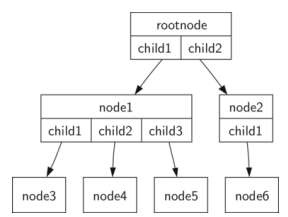
\includegraphics[scale=.5]{images/tree_edges_nodes.png}
% \end {center}

